\documentclass{article}

% Language setting
% Replace `english' with e.g. `spanish' to change the document language
\usepackage[french]{babel}
\usepackage[fleqn]{amsmath} % Aligner les équations à gauche


% Set page size and margins
% Replace `letterpaper' with`a4paper' for UK/EU standard size
\usepackage[letterpaper,top=2cm,bottom=2cm,left=3cm,right=3cm,marginparwidth=1.75cm]{geometry}

% Useful packages

\usepackage{amsmath}
\usepackage{graphicx}
\usepackage{subcaption}
\usepackage[colorlinks=true, allcolors=blue]{hyperref}

\title{TD 8 - Magnétostatique}
\author{IPESUP - PC }
\date{12/11/2024}
\begin{document}
\maketitle

\section{Rappels de cours}

Force de Lorentz subie par une particule chargée ($q$), de vitesse $v$ dans un champ magnétique $\vec{B}$: $\vec{F} = q \vec{v} \wedge \vec{B}$. \\


\textbf{Théorème de Maxwell-Ampère}: \\

Soit $\Gamma$ une courbe \textbf{fermée}, orientée. \\

$ \int_\Gamma \vec{B} \cdot  d \vec{l} = \mu_0 i_e$\\


Forme locale: $\vec{rot}(\vec{B}) = \mu_0 \vec{j}$. \\[0.2cm]

\textbf{Equation de Maxwell-Thomson:  }\\

${div}(\vec{B}) = 0$ \\[0.2cm]


\textbf{Force de Laplace:}\\
La force élémentaire de Laplace exercée sur un volume $d \tau$ de conducteur, soumis au champ magnétique $\vec{B}$, a pour expression : $d\vec{F}_L = \vec{j} \wedge \vec{B} d\tau$ \\

La force élémentaire de Laplace exercée sur une portion élémentaire de fil $d\vec{l}$ parcouru par un courant $i$ champ magnétique $\vec{B}$, a pour expression $d\vec{F}_L = i d \vec{l} \wedge \vec{B}$  \\[0.2cm]

\textbf{Propriétés: }
\begin{enumerate}
  \item Les plans de symétrie de la distribution de courant sont des champs d'antisymétrie du champ magnétique. 
  \item Le flux du champ magnétique à travers une section d'un tube de champ est constant.\\[0.2cm]
\end{enumerate}


\textbf{Propriétés des lignes de champ: }

\begin{enumerate}
  \item Les lignes de champ sont des courbes qui s'enroulent autour des courants et sont fermées. 
  \item Les lignes de champ sont orientées dans le sens positif par rapport au courant (règle de
  la main droite ou du tire bouchon). 
  \item Les lignes de champ sont plus resserrées là où le champ magnétique est plus intense. Lorsque les lignes de champ sont parallèles, le champ est donc uniforme.\\[0.2cm]
\end{enumerate}

\textbf{Dipôle magnétique: }\\

Moment magnétique d'une boucle de courant: $\vec{\mathcal{M}} = i \vec{S}$, avec $\vec{S}$ le vecteur surface orienté dans le sens de la circulation du courant. \\
Dans un champ magnétique uniforme, les actions de Laplace s'exeçant sur une boucle de courant indéformable ont un moment égal à $\Gamma = \vec{\mathcal{M}} \wedge \vec{B}$ et une résultante nulle.  \\
L'énergie potentielle d'un dipôle rigide dans un champ magnétique est donnée par $\vec{\mathcal{M}} \cdot \vec{B}$ \\

\textbf{Capacités exigibles: }
\begin{enumerate}
  \item Théorème de Maxwell-Ampère, énoncé en forme intégrale et locale. 
  \item Champ magnétique créé par un fil rectiligne infini parcouru par un courant $i$.
  \item Champ créé par un conducteur cylindrique parcouru par un courant uniforme. 
  \item Champ créé par un solénoïde infini. 
  \item Déterminer le moment magnétique de l'atome d'hydrogène et donner la valeur du facteur gyromagnétique. 
  \item Actions des forces de Laplace et énergie d'un dipôle magnétique dans un champ magnétique.
  \item Expliquer l'effet Hall et retrouver la valeur de tension de Hall. 
  \item Décrire l'expérience de Stern et Gerlach.
\end{enumerate}

\section{Calcul de champ: }


% Dans l'épisode 1 de la saga Pokémon, Pikachu utilise fatal foudre pour faire fuir un vol de Roucools. 
% En supposant que Pikachu est sur le sol, isolant, au moment de l'attaque, calculer le champ magnétique dans tout l'espace. 
On considère un fil semi infini (pour les $z<0$), parcouru par un courant $i$ et orienté selon $+\vec{u}_z$.
Le demi-espace $z>0$ est conducteur. 
Déterminer le champ magnétique en tout point du demi-espace $z>0$.


\section{Jonction entre deux conducteurs: }

On considère la jonction entre deux conducteurs par deux plans d'abscisse $x=a/2$ et $x=-a/2$.
Entre ces deux plans circulent des charges, donnant lieu à un courant de densité pouvant être modélisé par $\vec{j}(x, y, z) = j_0  sin(\frac{\pi x }{a})\vec{e}_y$.
Déterminer le champ dans tout l'espace. \\[0.1cm]

\section{Boule de Rowland: }
On considère une boule uniformément chargée en volume, de rayon $R$ et de densité volumique $\rho$, en rotation autour de l'axe $(Oz)$, avec une vitesse angulaire $\omega$ constante. 
Déterminer $\vec{j}$, le vecteur de densité de courant, puis l'intensité traversant un demi disque de rayon $R$ s'appuyant sur $(Oz)$. 


\section{Champ au voisinage de l'axe d'un spire}

On considère une spire circulaire de rayon $a$ parcourue par un courant $i$.

\begin{enumerate}
  \item Justifier que sur un point de l'axe $(Oz)$, le champ magnétique est de la forme $\vec{B} = B_0(z) \vec{u_z}$
  \item On se place près de l'axe, déterminer une approximation de $\vec{B}(M)$ au deuxième ordre. 
\end{enumerate}
% \section{Paradoxe de Feynman: }

% On considère un solénoïde semi-infini de rayon $a$, posé sur une plaque pouvant pivoter autour de l'axe $(Oz)$ et parcouru par un courant $ i(t).$, avec $i(t) = I$, pour $t<0$.  
% Sur la plaque sont disposées $N$ charges $q>0$ à une distance $b$ de l'axe. 
% A $t=0$, on coupe le courant. 
% Que se passe-t-il ? 

% \section{Situation qu'on rencontre dans la vie de tous les jours}

% On considère un cylindre chargé uniformément en surface et pouvant tourner autour de son axe horizontal. 
% Une masse M est suspendue au bout d'un fil inextensible enroulé autour du cylindre. 
% On lâche la masse, déterminer $\omega(t)$ la vitesse angulaire du cylindre. \\[2cm]

\begin{figure}[h]
  \centering
  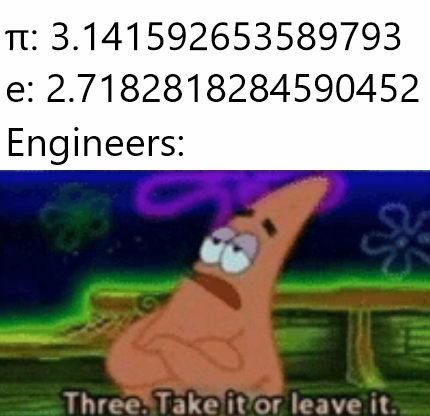
\includegraphics[width=0.3\textwidth]{meme.png}
\end{figure}




\end{document}

